\section{Empirical study on eleven data settings}\label{sec:empirical}

\subsection{Data, models and protocol}
We use eleven settings built from ten public binary classification data sets available on OpenML (Table~\ref{tab:data}; details in Supplementary Section~\SIref{app:data}). In five settings the group is a protected attribute: sex or race in Adult, age below 30 in Bank Marketing, sex in the credit-card default data and race in the law-school admission data. In the other six the group is an arbitrary split of the first numeric feature at its median, removed from the features; these settings have no fairness meaning but cover a wider range of prediction structures. A twelfth candidate (Nomao) was excluded because its arbitrary group contains no positive instances.

Each data set is split once into a training part (60\%) and a pool (40\%); the Electricity data (45,312 rows) were first subsampled to 30,000, while Adult and Bank Marketing are used in full. Nine classifiers are trained on the training part with scikit-learn: logistic regression with default and with strong regularisation, decision trees of depth 3 and 12, a random forest, histogram gradient boosting, 25-nearest neighbours, Gaussian naive Bayes and a multilayer perceptron. Their predictions and predicted probabilities on the pool, together with the group attribute, are all the design uses. The pool labels play two roles: they answer label queries, and they define the true values of the estimands, so that the error of every estimate is known exactly.

For each setting and budget $L\in\{250,500,1000,2000\}$ with $L\le N/4$ (35 setting--budget cells), we draw 200 independent labelled samples under each design and compute the $3\binom{9}{2}=108$ comparison estimands of \eqref{eq:theta}. The efficiency of a design is the ratio of the mean squared error under SRS to that under the design, computed for each estimand and summarised by the median over estimands; an efficiency of 4 means that SRS needs about four times as many labels for the same accuracy. Estimands whose true value is identically degenerate in the pool (for example when no model pair disagrees in a group) are excluded; this affects 51 of 108 estimands in the law-school setting only. Efficiencies are computed over the samples in which both designs give finite estimates; SRS produced an undefined estimate (no sampled positive in a group) in at most 0.5\% of its samples and the stratified designs never did. The designs are those of Section~\ref{sec:design}: SRS, SRS-DIF, GROUP, GROUP-DIF, PATTERN (plain estimator) and the proposed PATTERN-DIF, together with a variant of PATTERN-DIF whose allocation uses the residual variances. SRS, GROUP and PATTERN use the same random seeds as the earlier plug-in study (\texttt{results/label\_efficiency.json}), so their samples coincide with it and their efficiencies agree except in law school, where that study used a different set of compared estimands. The code and all results are in the repository (\texttt{experiments/label\_efficiency\_dif.py}, \texttt{results/label\_efficiency\_dif.json}).

\begin{table}[t]\centering\small
\caption{Data settings. Pool: size of the held-out pool from which labels are drawn. $P_0,P_1$: positives in each group. Disagreement: share of pool instances on which two of the three most accurate models disagree, averaged over the three pairs. Groups marked ``arbitrary'' are median splits of a numeric feature.}\label{tab:data}
\begin{tabular}{lcrrrr}\toprule
Setting & Group & Pool $N$ & Positives $P_0$ & Positives $P_1$ & Disagreement \\\midrule
Adult (sex) & sex & 19537 & 3963 & 712 & 0.053 \\
Adult (race) & race & 19537 & 4249 & 426 & 0.047 \\
Bank marketing & age & 18085 & 1753 & 363 & 0.045 \\
Credit card & sex & 12000 & 1148 & 1506 & 0.030 \\
Law school & race & 8320 & 2038 & 640 & 0.000 \\
MAGIC & arbitrary & 7608 & 1084 & 1591 & 0.049 \\
EEG eye state & arbitrary & 5992 & 1183 & 1506 & 0.086 \\
Phoneme & arbitrary & 2162 & 388 & 247 & 0.095 \\
Spambase & arbitrary & 1841 & 490 & 235 & 0.043 \\
Churn & arbitrary & 2000 & 149 & 134 & 0.041 \\
Electricity & arbitrary & 12000 & 2582 & 2488 & 0.086 \\
\bottomrule\end{tabular}
\end{table}

\subsection{Efficiency}
Table~\ref{tab:efficiency} gives the efficiency of every design in every cell, Table~\ref{tab:decomposition} summarises it by budget and Figure~\ref{fig:efficiency} shows it as a function of the budget and of the disagreement rate. Across settings, the median efficiency of PATTERN-DIF relative to SRS is 5.8 at $L=250$ (eleven settings), 6.3 at $L=500$ (ten), 6.9 at $L=1000$ (eight) and 15.5 at $L=2000$ (six); without the degenerate law-school setting the medians are 5.5, 5.8, 6.0 and 9.4. SRS thus needs between five and sixteen times as many labels to match PATTERN-DIF, and the lowest efficiency in any cell outside law school is 3.5. The medians over settings rise with the budget partly because the set of settings changes (only the larger pools allow the larger budgets): on the seven non-degenerate settings that are present at $L=250$, 500 and 1000 the medians of PATTERN-DIF are 5.3, 5.3 and 6.0 (3.5, 3.8 and 4.4 for PATTERN). Within each of these seven settings the efficiency does increase with the budget (a median increase of 23\% from $L=250$ to $L=1000$), because a larger budget labels a larger share of the small disagreement strata, where the variance of the comparisons is concentrated. The increase is moderate except at $L=2000$, where the remaining settings are those with the largest pools and the strongest gains.

\paragraph{Where the gain comes from.} Table~\ref{tab:decomposition} separates the two ingredients, and the design is the larger. Under the difference estimator, moving from simple random sampling to the PATTERN strata multiplies the efficiency by 3.3 to 8.6 (PATTERN-DIF against SRS-DIF), and under the plain estimator by 3.7 to 7.3 (PATTERN against SRS). The estimator contributes 1.3 to 1.65 on top of the PATTERN design (PATTERN-DIF against PATTERN, better in 34 of 35 cells), but only 1.8 to 2.0 on top of simple random sampling (SRS-DIF against SRS). The two ingredients are complementary, and neither accounts for the whole gain. Stratifying by group alone gives almost no gain under the plain estimator (median 1.04 to 1.05 at the first three budgets and 1.25 at $L=2000$, where it is 1.0 without law school) and 2.1 to 2.7 with the difference estimator, which is essentially the value of the proxy correction. The variance of a contrast between two models is driven by the instances on which they disagree, and these are spread over both groups.

\paragraph{By estimand.} Efficiency differs by estimand. For PATTERN-DIF the medians over settings at the four budgets are 5.8, 5.3, 8.9 and 17.0 for $\theta^{\mathrm{TPR}}$, 7.6, 8.5, 8.4 and 20.6 for $\theta^{\mathrm{FPR}}$, and 3.5, 4.1, 4.4 and 5.7 for $\theta^{\mathrm{ERR}}$. The fairness contrasts gain more than the error contrast because they depend on the rarest cells (positives or negatives in the minority group). In Adult with race as the group, at $L=1000$, the efficiencies are 23.9 for $\theta^{\mathrm{TPR}}$, 20.6 for $\theta^{\mathrm{FPR}}$ and 3.7 for $\theta^{\mathrm{ERR}}$. For the pairs formed by the three most accurate models, the comparisons most likely to matter in practice, the median efficiency of PATTERN-DIF is 5.8, 6.8, 6.6 and 10.5 at the four budgets (3.3, 4.2, 3.9 and 6.2 for PATTERN).

\begin{figure}[t]\centering
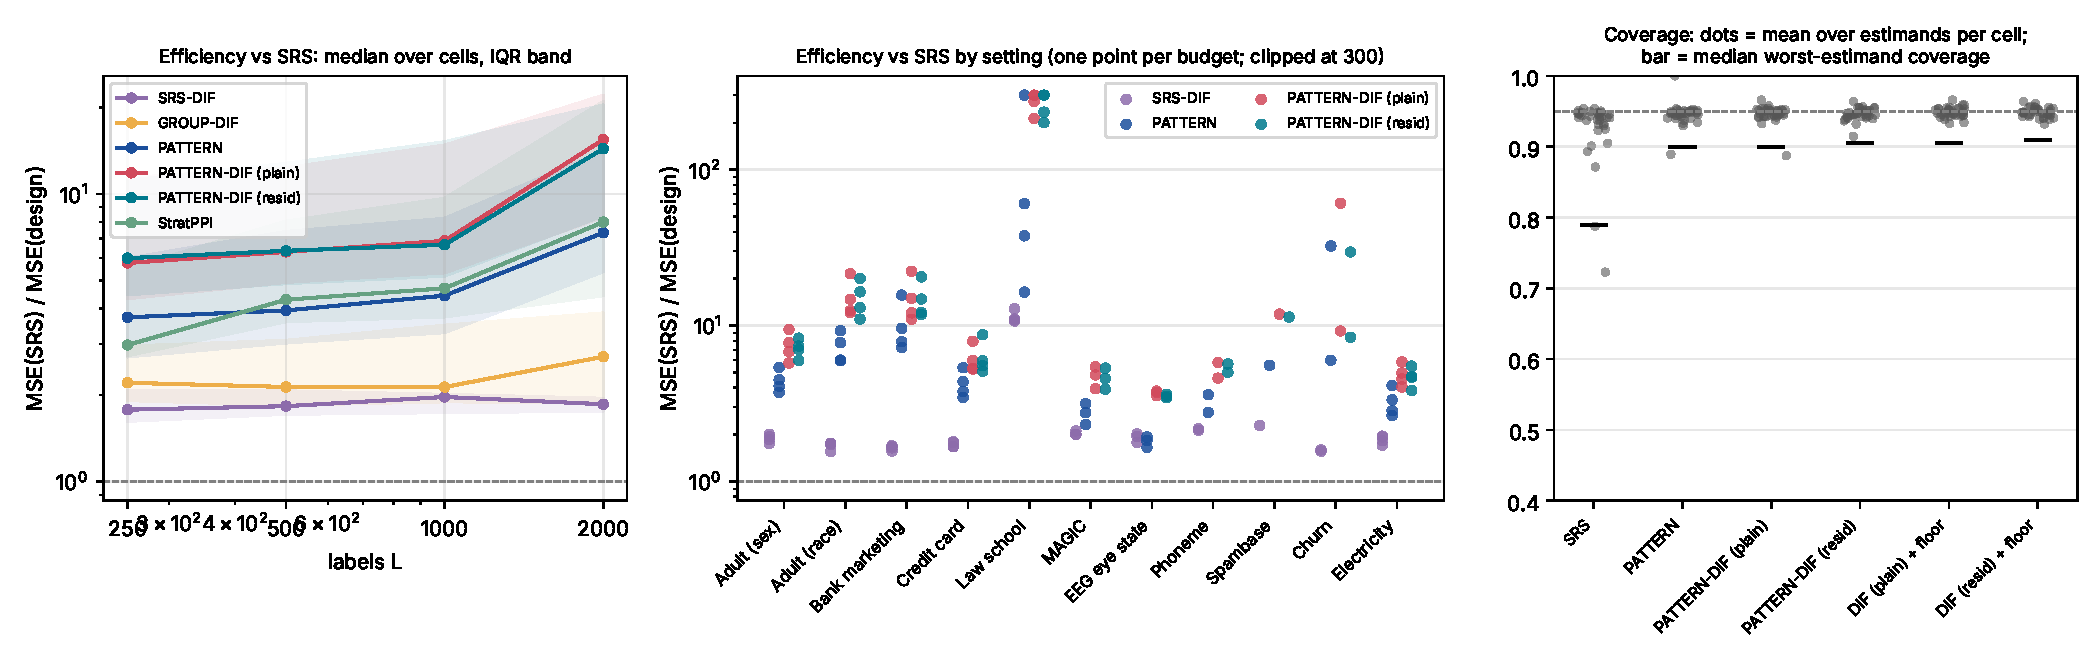
\includegraphics[width=\textwidth]{figures/efficiency_dif.pdf}
\caption{Efficiency of the designs relative to SRS (median over the comparison estimands) as a function of the label budget and of the disagreement rate; see Table~\ref{tab:efficiency} for the numbers.}\label{fig:efficiency}
\end{figure}

\begin{table}[t]\centering\small
\caption{Decomposition of the efficiency gain by budget (median over settings of the cell medians). Each row is a ratio of mean squared errors. ``DIF resid vs DIF plain'' compares the residual-variance allocation with the allocation used by default.}\label{tab:decomposition}
\begin{tabular}{lrrrr}\toprule
Step (MSE ratio) & $L=250$ & $L=500$ & $L=1000$ & $L=2000$ \\\midrule
SRS-DIF vs SRS & 1.78 & 1.83 & 1.97 & 1.86 \\
PATTERN vs SRS & 3.72 & 3.94 & 4.43 & 7.33 \\
PATTERN-DIF vs PATTERN & 1.65 & 1.54 & 1.51 & 1.31 \\
PATTERN-DIF vs SRS-DIF & 3.28 & 3.29 & 3.72 & 8.57 \\
PATTERN-DIF vs SRS & 5.76 & 6.29 & 6.87 & 15.5 \\
DIF resid vs DIF plain & 1.01 & 0.97 & 0.96 & 1.00 \\
\bottomrule\end{tabular}

\end{table}

\subsection{Efficiency and disagreement}
The gain is larger when the models disagree less (Figure~\ref{fig:efficiency}). The Spearman correlation between the disagreement rate of the three best models and the efficiency of PATTERN-DIF is $-0.58$ at $L=250$ (ten settings), $-0.53$ at $L=500$ (nine) and $-0.71$ at $L=1000$ (seven), excluding law school ($-0.68$, $-0.66$ and $-0.81$ with it). The three settings with the highest disagreement (EEG, electricity and phoneme, 8.6\% to 9.5\%) have the smallest gains, between 3.7 and 5.8 at $L=500$. The relation is inexact, since efficiency also depends on the size of the minority cells and on the magnitude of the contrasts (Section~\ref{sec:theory}; checked in Supplementary Section~\SIref{sec:simulation}).

Two settings are atypical. In the law-school data all nine models predict almost identically (the three best models disagree on fewer than 0.01\% of instances); the design then labels almost every disagreement instance and the contrasts are estimated nearly exactly, so the efficiency ratios (about 270 at $L=500$, 510 at $L=1000$ and above $10^{4}$ at $L=2000$) show only that SRS wastes labels on agreements. In the churn data (a pool of 2,000) the efficiency of PATTERN-DIF at $L=500$ is 61, driven by contrasts of false positive rates and of errors that are concentrated in very few instances.

\begin{table*}[p]\centering\footnotesize
\caption{Efficiency (ratio of mean squared errors, median over estimands) by setting and budget. DIF plain: PATTERN-DIF with the default allocation; DIF resid: with the residual-variance allocation; StratPPI: stratified prediction-powered inference (Section~\ref{sec:baselines}). ``vs PATTERN'': PATTERN-DIF relative to the plain estimator under the same design. The last three columns are the efficiencies of PATTERN-DIF by estimand type. Bold marks the best of the two PATTERN-DIF variants.}\label{tab:efficiency}
\begin{tabular}{lrrrrrrrr rrr}\toprule
Setting & $L$ & \multicolumn{6}{c}{Efficiency vs SRS} & vs PATTERN & \multicolumn{3}{c}{PATTERN-DIF (plain) by estimand} \\
 & & SRS-DIF & GROUP-DIF & PATTERN & DIF plain & DIF resid & StratPPI & DIF plain & $\theta^{TPR}$ & $\theta^{FPR}$ & $\theta^{ERR}$ \\\midrule
Adult (sex) & 250 & 1.75 & 2.20 & 3.72 & 5.76 & \textbf{5.98} & 3.28 & 1.37 & 8.68 & 7.59 & 3.50 \\
 & 500 & 1.86 & 1.95 & 4.08 & 6.80 & \textbf{7.02} & 4.07 & 1.49 & 9.30 & 8.20 & 3.83 \\
 & 1000 & 2.01 & 1.91 & 4.49 & \textbf{7.76} & 7.39 & 4.71 & 1.51 & 11.8 & 8.75 & 4.28 \\
 & 2000 & 1.94 & 1.87 & 5.39 & \textbf{9.42} & 8.30 & 5.54 & 1.32 & 11.7 & 11.8 & 5.03 \\
\addlinespace
Adult (race) & 250 & 1.56 & 3.31 & 5.96 & \textbf{12.1} & 11.0 & 5.46 & 1.65 & 18.1 & 15.4 & 2.96 \\
 & 500 & 1.73 & 3.33 & 6.02 & 12.4 & \textbf{13.0} & 6.95 & 1.44 & 17.5 & 14.9 & 3.44 \\
 & 1000 & 1.76 & 3.36 & 7.78 & 14.7 & \textbf{16.5} & 8.52 & 1.48 & 23.9 & 20.6 & 3.70 \\
 & 2000 & 1.75 & 3.52 & 9.28 & \textbf{21.5} & 20.0 & 10.4 & 1.30 & 37.5 & 29.3 & 4.36 \\
\addlinespace
Bank marketing & 250 & 1.57 & 3.84 & 7.22 & 11.0 & \textbf{11.8} & 7.80 & 1.44 & 11.0 & 18.6 & 5.05 \\
 & 500 & 1.64 & 3.99 & 7.87 & 12.1 & \textbf{12.1} & 10.3 & 1.45 & 12.1 & 24.7 & 6.31 \\
 & 1000 & 1.67 & 3.90 & 9.60 & \textbf{15.0} & 14.8 & 13.1 & 1.43 & 15.6 & 38.9 & 6.56 \\
 & 2000 & 1.69 & 3.97 & 15.7 & 22.3 & 20.5 & \textbf{24.5} & 1.32 & 22.3 & 79.9 & 9.18 \\
\addlinespace
Credit card & 250 & 1.67 & 1.86 & 3.45 & \textbf{5.31} & 5.09 & 2.58 & 1.26 & 3.55 & 7.18 & 4.27 \\
 & 500 & 1.80 & 1.81 & 3.79 & 5.26 & \textbf{5.53} & 3.52 & 1.29 & 4.81 & 7.84 & 4.30 \\
 & 1000 & 1.67 & 1.68 & 4.37 & \textbf{5.98} & 5.94 & 3.71 & 1.42 & 5.90 & 8.01 & 5.00 \\
 & 2000 & 1.78 & 1.91 & 5.36 & 7.93 & \textbf{8.72} & 4.06 & 1.20 & 5.43 & 10.5 & 6.32 \\
\addlinespace
Law school & 250 & 10.9 & 22.2 & 16.4 & \textbf{$>$100} & $>$100 & 31.8 & 10.7 & $>$100 & $>$100 & $>$100 \\
 & 500 & 12.8 & 19.7 & 37.6 & \textbf{$>$100} & $>$100 & 52.4 & 9.46 & $>$100 & $>$100 & $>$100 \\
 & 1000 & 11.0 & 21.4 & 60.4 & \textbf{$>$100} & $>$100 & 78.4 & 8.26 & $>$100 & $>$100 & $>$100 \\
 & 2000 & 10.7 & 20.4 & \textbf{$>$100} & $>$100 & $>$100 & $>$100 & 0.00 & $>$100 & $>$100 & $>$100 \\
\addlinespace
MAGIC & 250 & 2.01 & 1.98 & 2.32 & \textbf{3.93} & 3.90 & 2.71 & 1.65 & 3.89 & 5.30 & 3.06 \\
 & 500 & 2.11 & 2.26 & 2.76 & \textbf{4.82} & 4.57 & 3.81 & 1.71 & 4.89 & 5.94 & 3.27 \\
 & 1000 & 2.01 & 2.10 & 3.16 & \textbf{5.43} & 5.33 & 4.69 & 1.61 & 4.73 & 6.75 & 4.60 \\
\addlinespace
EEG eye state & 250 & 1.78 & 1.96 & 1.65 & \textbf{3.55} & 3.51 & 2.71 & 1.93 & 3.80 & 4.06 & 2.98 \\
 & 500 & 1.94 & 2.00 & 1.83 & \textbf{3.73} & 3.44 & 3.33 & 1.82 & 4.23 & 3.99 & 3.15 \\
 & 1000 & 2.02 & 2.16 & 1.93 & \textbf{3.80} & 3.61 & 3.68 & 1.91 & 4.06 & 4.86 & 3.04 \\
\addlinespace
Phoneme & 250 & 2.13 & 2.29 & 2.77 & 4.60 & \textbf{5.02} & 2.98 & 1.77 & 4.68 & 6.74 & 3.19 \\
 & 500 & 2.18 & 2.41 & 3.60 & \textbf{5.79} & 5.67 & 4.51 & 1.78 & 5.66 & 8.71 & 4.36 \\
\addlinespace
Spambase & 250 & 2.29 & 2.61 & 5.55 & \textbf{11.8} & 11.3 & 5.56 & 2.19 & 16.1 & 20.0 & 5.69 \\
\addlinespace
Churn & 250 & 1.56 & 1.49 & 5.99 & \textbf{9.22} & 8.41 & 2.96 & 1.42 & 5.77 & 10.3 & 9.48 \\
 & 500 & 1.59 & 1.78 & 32.4 & \textbf{60.8} & 29.6 & 8.42 & 1.28 & 4.46 & 70.6 & 77.1 \\
\addlinespace
Electricity & 250 & 1.83 & 1.84 & 2.65 & \textbf{4.04} & 3.83 & 2.76 & 1.63 & 4.88 & 5.26 & 2.97 \\
 & 500 & 1.71 & 1.78 & 2.84 & 4.54 & \textbf{4.66} & 3.40 & 1.59 & 4.82 & 5.42 & 3.20 \\
 & 1000 & 1.93 & 1.85 & 3.34 & \textbf{4.97} & 4.72 & 3.74 & 1.51 & 5.01 & 6.27 & 4.07 \\
 & 2000 & 1.95 & 1.85 & 4.12 & \textbf{5.85} & 5.49 & 3.92 & 1.44 & 5.54 & 8.34 & 5.12 \\
\bottomrule\end{tabular}

\end{table*}

\subsection{Inference and decisions}
Table~\ref{tab:inference} reports the coverage of nominal 95\% intervals. The mean coverage of the PATTERN-DIF intervals is 0.940 at $L=250$, 0.946 at $L=500$ and between 0.950 and 0.952 at larger budgets; for PATTERN with the plain estimator it is 0.938, 0.944, 0.950 and 0.956. Under SRS it is 0.911 to 0.942, and the worst-covered estimand has coverage as low as 0.10 at $L=250$, because SRS samples often contain no disagreement instance in a small cell and then give a zero standard error. The worst-covered estimand under PATTERN-DIF has coverage 0.59 at $L=250$ (in law school), 0.84 at $L=500$ and 0.89 to 0.90 at larger budgets. The intervals are therefore adequate on average from 250 labels on, and for every estimand from about 1,000 labels on (worst-estimand coverage 0.89 to 0.90, about the minimum that chance alone gives over 108 estimands with 200 replicates). They fail in small cells at small budgets, where a stratum in which every sampled label is the same gives a variance estimate of exactly zero. A safeguard that replaces the zero variance of such a stratum by its variance under the proxy (a ``variance floor'', Section~\ref{sec:ablations}) raises the worst-estimand coverage at $L=250$ from 0.59 to 0.82 and keeps the mean at 0.946; a more conservative version raises the mean to 0.98. The floor was designed after seeing this failure on these pools, so the improvement is in-sample. At small budgets we report both the plain Wald and the floor intervals.

\begin{table*}[t]\centering\small
\caption{Quality of inference by budget. Mean: coverage of nominal 95\% intervals averaged over estimands and cells; worst: the lowest coverage of any estimand in any cell. ``+ floor'': Wald intervals with the zero-variance safeguard. Fail: largest share of samples with an undefined estimate (SRS only).}\label{tab:inference}
\resizebox{\textwidth}{!}{\begin{tabular}{rrrrrrrrrrrrrrrrr}\toprule
$L$ & Cells & \multicolumn{2}{c}{SRS} & \multicolumn{2}{c}{PATTERN} & \multicolumn{2}{c}{PATTERN-DIF (plain)} & \multicolumn{2}{c}{PATTERN-DIF (resid)} & \multicolumn{2}{c}{DIF (plain) + floor} & \multicolumn{2}{c}{DIF (resid) + floor} & \multicolumn{2}{c}{PATTERN + floor} & Fail \\
 & & mean & worst & mean & worst & mean & worst & mean & worst & mean & worst & mean & worst & mean & worst & (max) \\\midrule
250 & 11 & 0.911 & 0.10 & 0.938 & 0.53 & 0.940 & 0.59 & 0.943 & 0.69 & 0.946 & 0.82 & 0.948 & 0.85 & 0.963 & 0.90 & 0.005 \\
500 & 10 & 0.923 & 0.28 & 0.944 & 0.82 & 0.946 & 0.84 & 0.944 & 0.85 & 0.948 & 0.84 & 0.945 & 0.85 & 0.959 & 0.89 & 0.000 \\
1000 & 8 & 0.938 & 0.71 & 0.950 & 0.89 & 0.952 & 0.90 & 0.949 & 0.90 & 0.952 & 0.90 & 0.950 & 0.90 & 0.959 & 0.91 & 0.000 \\
2000 & 6 & 0.942 & 0.53 & 0.956 & 0.89 & 0.950 & 0.89 & 0.952 & 0.90 & 0.950 & 0.89 & 0.952 & 0.90 & 0.957 & 0.89 & 0.000 \\
\bottomrule\end{tabular}}

\end{table*}
